 \documentclass[10pt]{extarticle}

%SOME USEFUL PACKAGES
\usepackage[portuguese]{babel}
\usepackage{extsizes}
\usepackage[reqno]{amsmath} % equation numbers on the right
\usepackage{amsmath}
\usepackage{amssymb}
\usepackage{amsthm}
\usepackage{amscd}
\usepackage{amsfonts}
\usepackage{graphicx}
\usepackage{dsfont}
\usepackage{fancyhdr}
\usepackage{enumerate}
\usepackage[utf8]{inputenc}
\usepackage{booktabs}
\usepackage{listings}
\usepackage[margin=1in]{geometry}
\usepackage[hypcap]{caption}
\usepackage{longtable}
\usepackage{etoolbox}
%\usepackage[alf]{abntex2cite}
\usepackage[siunitx]{circuitikz}
\usepackage{tikz}
\usepackage{enumitem}
\usepackage{algpseudocode}
\usepackage{algorithm}


\usepackage{verbatim}
\usepackage{float}
\usepackage{indentfirst}

%HEADER
\pagestyle{fancy}\lhead{Vinícius Julião Ramos} \rhead{DCC605 - Sistemas Operacionais - 2020.2}
\chead{{\large{\bf }}} \lfoot{} \rfoot{\bf \thepage} 
\cfoot{}


\title{ \textsc{Universidade Federal de Minas Gerais} \\
\textsc{Departamentode Ciência da Computação} \\
\bigskip TP2 -- Simulação de um sistema de memória virtual}

\author{Vinícius Julião Ramos \\ \normalsize{viniciusjuliao@dcc.ufmg.br}}

\date{\today}

\begin{document}
\maketitle

\begin{abstract}
O trabalho aqui apresentado consiste na elaboração de algoritmos de
reposição para tabela de páginas.
Tais algoritmos funcionarão num ambiente simulado, no qual serão dados: o
tamanho total da tabela, o tamanho de cada página e  uma lista de endereços de
que representam acessos à memória.
Sendo assim, a partir de tais acessos, os algoritmos implementados terão o
trabalho de validar determinado endereço encontra-se disponível.
Em caso negativo, há a necessidade de tornar aquele endereço disponível e
isso pode levar à exclusão de alguma outra página (alocada anteriormente),
uma vez que há uma limitação de espaço.
Quatro algoritmos foram desenvolvidos e tiveram seus desempenhos comparados,
sendo que um, dentre estes quatro, foi proposto pelo aluno.
Os outros três métodos de reposição desenvolvidos por este trabalho foram dados
apresentados pela especificação.
\end{abstract}
    
\section{Introdução}
Sistemas operacionais, precisam prover acesso à memória para os diversos
programas em execução.
Porém, memória é um recurso limitado e que deve ser gerenciado de maneira a
atender todos os processos em execução.
Essa tarefa necessita de um mecanismo capaz de realizar tal controle,
permitindo que programas acessem à memória e também ao disco, entretanto
abstraindo do processo em execução a necessidade de identificar se determinado
endereço de memória está no disco ou na memória volátil da máquina.
Tal função é conhecida como virtualização de memória e nisso encontra-se a
necessidade de um algoritmo que crie uma tabela na qual liste as páginas que um
processo possui armazenadas em memória, ou em disco.
Essa tabela possui um espaço limitado, então se um endereço (virtual)
encontra-se em disco, cabe ao mecanismo de virtualização a busca desses dados e
a colocação na memória física.

Quando determinado programa já ocupou todo o espaço reservado para a própria
execução, é necessário iniciar o salvamento dos dados em disco.
Essa ação leva à necessidade de realizar trocas entre o disco e a memória
volátil; sendo que o responsável pela troca é o algoritmo de reposição.
Por fim, para este trabalho, foi proposto o desenvolvimento de quatro
algoritmos de reposição: \textit{LRU}, \textit{Second Chance}, \textit{FIFO}
e um quarto algoritmo \textit{Custom}, que seria proposto pelo próprio aluno.
Dado o ambiente virtual do trabalho, tomaremos métricas diferentes do tempo de
execução para avaliar o desempenho de cada um dos métodos.
O ambiente simulado não executa leitura e escrita em disco assim como acontece
no ambiente real, portanto, aqui o tempo não é um grande fator de impacto.
Logo, as métricas avaliadas consistem na quantidade de páginas não encontradas
na memória volátil (\textit{page-faults}) e a quantidade de páginas sujas 
(\textit{dirty}) -- tais métricas identificam a quantidade de leituras e
escritas feitas no disco, respectivamente.

Os códigos apresentados por esse trabalho foram desenvolvidos na linguagem C e
testados no sistema operacional Ubuntu 16.04 e 18.04.
Uma vez que a linguagem permite a criação de tipos abstratos de dados, tal
conceito fora aplicado para instanciar as entidades necessárias no controle dos
métodos de substituição.
\newpage

\section{Modelagem e Decisões de Projeto}
%  Modelagem e decisões de projeto

A principal decisão a cerca deste trabalho foi em todo da definição de uma
estrutura de dados que modelasse a tabela de páginas.
Dentre as opções propostas pela especificação, escolheu-se aquela que permitiu
uma rápida implementação.
Entretanto, um bom nível de abstração de código foi criado, logo, caso
haja a necessidade de mudar a estrutura de dados utilizada, tal ação não gerará
uma grande mudança no código.
Para a tabela de páginas utilizamos um \textit{array} de uma TAD do tipo
\texttt{pageattr}, em que cada elemento desse tipo abstrato de dados possui uma
série de atributos utilizados pelos algoritmos de substituição.
Tal \textit{array} possui $n$ elementos, em que $n$ é o numero máximo de páginas
de tamanho $k$ que podem ser endereçadas por números binários de 32 bits.
Ou seja, imagine um exemplo em que uma página possua $k = 4$ Kilo Bytes, então,
uma vez que cada byte da memória é endereçado por um número de 32 bits, temos:

$$
n = 2^{32} \div 4096 = 2^{32} \div 2^{12} = 2^{32-12} = 2^{20}
$$

Uma outra conta pode ser feita de forma que, dado o tamanho de página $k$ temos
$n$ igual a:
$$
n = 2^{32 - \log_2{k}}
$$


% Falar da existência de uma tabela que possui 2^(32- log_2(page_size))
% a  estrutura princial é o pageattr que possui algumas informações:
%   - uma flag `is_valid`, uma flag `dirty`, dois ponteiros: `next` e `prev`
Utilizando de tal abordagem, podemos validar se determinada página está ou não
na tabela de páginas em tempo $O(1)$, uma vez que \texttt{pageattr} possui um
bit identificador \texttt{is\_valid} que denota a presença ou ausência daquela
página na memória.
Dado um endereço qualquer, o endereço de sua própria página é obtido através de
uma operação de \textit{shifting} de bits, em que $\log_2k$ bits serão "shiftados"
de forma a remover os bits menos significativos.
Este valor de $k$ é o mesmo dado pelo tamanho da página em Bytes.
Além do bit identificador \texttt{is\_valid}, o TAD \texttt{pageattr} possui os
outro seguintes atributos:
\begin{itemize}
    \item \texttt{dirty} -- Um bit identificador de \textit{dirty pages}, ou
    seja, valida se uma página já recebeu alguma operação de escrita.
    \item \texttt{next} e \texttt{prev} -- ponteiros para referenciar elementos
    vizinhos.
    Uma vez que a maior parte dos métodos consiste na construção de sequências,
    esses ponteiros são necessários mara marcar os elementos vizinhos entre si
    e caracterizar as listas nos métodos \textit{FIFO}, \textit{Second Chance}
    e \textit{LRU}.
    \item \texttt{last\_operation} -- Armazena um caractere com a informação da
    ultima operação recebida naquela página.
    Essa informação é usada para a impressão do relatório ao final da execução
    do programa.
\end{itemize}


% organização do código:
% - Main define 5 etapas principais:
%   1. leitura da entrada
%   2. ... 5.
%   Falar tmb das funções aplicadas a cada um dos algoritmos de substituição
%     O uso de orientação a objetos seria ideal nesses casos, dada a semelhança
%     que os códigos possuem, poderia-se criar interfaces.
% - Utils:
%   - impressão dos stats
%   - leitura do arquivo -> falar brevemente sobre a questão da resolução de ambiguidades
%     ao ler a entrada de uma maneira incorreta.
% - Pagetable
%   - define as estruturas e funções utilizadas na manipulação da tabela de páginas.
O código principal foi organizado em quatro etapas: (1) Abertura do
arquivo de entradas, (2) alocação de memória para as estruturas de dados
utilizadas, (3) execução do algoritmo especificado pelos argumentos, (4)
exibição do relatório de execução.
Dentro da terceira etapa encontra-se a leitura do arquivo contendo os endereços de
memória, mas esse fato será abordado mais adiante.
Todas essas etapas estão expressas no arquivo \texttt{main.c}, sendo que cada
algoritmo de substituição corresponde a uma função dentro deste mesmo arquivo.
É importante ressaltar a grande semelhança no código de cada um dos métodos de
substituição, e isso permite vislumbrar o uso de orientação a objetos na qual
é possível definir uma \textit{Interface} que padronize os métodos que serão
chamados ao encontrar um \textit{page fault} ou dada a necessidade de
reescrever uma \textit{dirty page} no disco.
Entretanto o uso da linguagem C não permite a aplicação desses conceitos, logo
a organização do código aqui proposto foi baseado em legibilidade e na
separação correta de funções comuns a algum tipo de execução.

Outros dois aquivos de código foram escritos a fim de organizar e separar
funcionalidades.
Os aquivos \texttt{page\_table.h} e \texttt{page\_table.c} contém a definição
das estruturas (TADs) responsáveis pela tabela de páginas, além das funções que
as gerenciam.
Já os arquivos \texttt{utils.h} e \texttt{utils.c} contém funções
para manipulação de entrada e saída, por exemplo a exibição do relatório final
de execução e também a leitura do arquivo de endereços de memória.
É importante ressaltar que na função de leitura do arquivo, foi necessário
tratar um possível erro de formatação; para que uma linha seja reconhecida
ela deve conter um número hexadecimal, seguido de um caractere espaço e um
outro caractere \texttt{R} ou \texttt{W}.
Caso não haja esse padrão, a linha é desconsiderada e tenta-se realizar a
leitura da próxima linha.
Enquanto não houver uma linha em concordância, as linhas serão
desconsideradas até encontrar o fim do arquivo.

% \begin{figure}[h]
% 	\begin{center}
% 		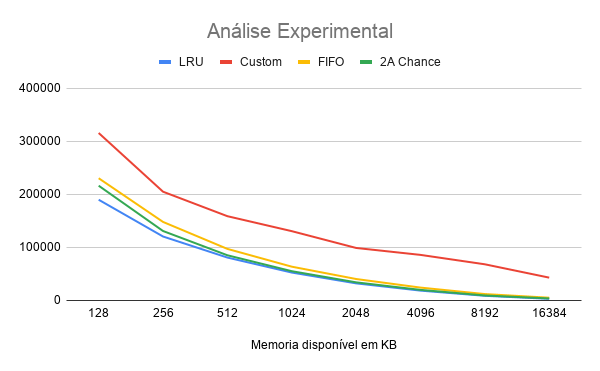
\includegraphics[scale=0.5]{Figuras/img1.png}
% 	\end{center}
% 	\caption{\label{fig:sudoku_grafo_colorido} Transformação do sudoku para grafo colorido.}
% \end{figure}

% \newpage

\section{Algoritmo de Substituição Próprio}
O algoritmo de substituição proposto por esse trabalho, foi baseado na criação
de um \textit{hashing} de endereços.
Dentre os argumentos recebidos pelo programa, temos a quantidade de memória
disponível ($q$) e o tamanho de cada página ($k$).
Então, sendo $l = q\div k$ a quantidade de páginas gerenciadas pelos métodos
de substituição, aplicamos uma função que mapeia qualquer endereço para um
número entre $0$ e $l-1$.
Assim, o método de substituição criado por esse trabalho, trabalhará com a
quantidade correta de páginas.
Esse hashing acontece de modo a aplicar uma operação booleana \textit{and}
bit a bit, entre o endereço da página requisitada e $l-1$.
Como $l$ será sempre um valor em potência de 2, temos que $l-1$, quando
transformado para a base 2, é um número preenchido apenas com 1.

Dessa maneira o hashing obtém os bits menos significativos do endereço de uma
página e assim, pode-se consultar nesse array de $l$ endereços, se determinada
página requisitada já está na memória ou não.
É importante informar que essa operação booleana é aplicada sobre o endereço
da página, ou seja, o endereço dado no arquivo de entrada passa por uma
transformação de shifting e assim é obtido o endereço da página, e só depois
disso aplica-se a operação \textit{and} bit a bit com $l-1$.
O hashing se dá da seguinte maneira:

\begin{algorithm}
    \caption{Hashing Transformation}\label{alg:transformation}
    \begin{algorithmic}[1]
    \Function{Hashing Transformation}{$Page\ Address\ PAddr, Pages\ Quantity\ l$}
        
    \Return $PAddr\ \&\&\ (l-1)$   
    \EndFunction
\end{algorithmic}
\end{algorithm}

Para melhor esclarecer, observe o seguinte exemplo:
Dada um programa com uma quantidade de memória disponível igual a 128 Kilo
Bytes, em que cada página possui 8 Kilo Bytes de memória disponível.
Nesse caso, teremos então $128 \div 8 = 16$ elementos na tabela de páginas,
logo $l = 16$.
Então suponha que o programa deseje acessar uma página $x$ em que o valor
decimal do endereço será $550$.
Portanto, dado um array $A$ que armazena os endereços das páginas disponíveis
na memória, em que o tamanho de $A$ é igual a $l$, poderemos mapear qualquer
endereço de página para uma posição em $A$ através da operação booleana
previamente citada.
Observe o mapeamento da página $x$:
$$
\langle\textit{and}\rangle\frac{x\ \ \rightarrow 550_{10}\ = 1000100110_2}{l-1 \rightarrow 15_{10} = 0000001111_2}
= 0000000110_2 = 12_{10}
$$

Por fim, a página de que tem o endereço igual a 550 será armazenada no índice
12 do vetor $A$, sendo que este vetor é indexado com o primeiro elemento na
posição 0.
Para executar o algoritmo criado por este trabalho, o argumento de execução
que contem o nome do método de reposição a ser executado dever ser 
\texttt{custom}.
% \newpage

\section{Análise Experimental}
Antes de demonstrar os comparativos entre os gráficos e avaliar qual dos
algoritmos possuiu melhor desempenho, vamos basear a questão do desempenho
pela quantidade de \textit{page faults} reportados pela execução.
Como não é possível obter métricas reais do tempo de execução da escrita e
leitura do disco, o número de páginas não encontradas na memória será o
norteador.
A justificativa vem do motivo de que: uma vez que uma página não é encontrada
na memória é necessário acessar o disco para carregar as informações daquela
página.
Além disso, quando um \textit{pag fault} é reportado, e o programa já faz uso
de toda a memória disponível para sua própria execução, são necessárias duas
operações: A possível escrita de uma \textit{dirty page} no disco e a leitura
da página solicitada.
Portanto, o uso da quantidade de paginas não encontradas na memória possui uma
forte justificativa para ser utilizada como métrica nesse ambiente simulado
que fora apresentado por este trabalho.


\subsection{Algoritmo customizado}
Nessa análise, foi executado todas as combinações disponíveis entre
\textit{Tamanho da Página}, \textit{Memória Disponível} e
\textit{Arquivo de Entrada}. Após obter os resultados, para cada valor
de \textit{Memória disponível}, calculou-se a média da quantidade de 
\textit{page faults} entre todos os pares de \textit{Tamanho da página}
e \textit{Arquivo de entrada}.
Ou seja, um ponto no gráfico da Figura \ref{fig:grafico1} corresponde a um valor fixo
do \textit{Algoritmo} e da \textit{Memoria Disponível} em contraste com
a média das execuções que variaram o valor dos outros dois argumentos.

\begin{figure}[h]
	\begin{center}
		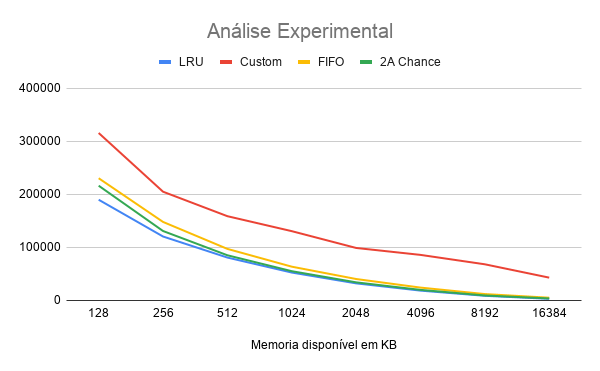
\includegraphics[scale=0.7]{Figuras/img1.png}
	\end{center}
	\caption{\label{fig:grafico1} }
\end{figure}

No gráfico da Figura \ref{fig:grafico1}, observamos que o algoritmo customizado
obteve uma quantidade de \textit{page faults} muito maior que os demais.
Podemos observar então, que esse tipo de hashing não é eficiente para essa aplicação
uma vez que muitos endereços possuem o conjunto dos bits menos significativos muito
próximos.
Possivelmente, uma abordagem melhor, seria criar tal hashing pelo bits mais
significativos, uma vez que valores de endereços com bits mais significativos
muito diferentes, identificam que tais endereços estão dispersos.
Entretanto, foi solicitado pelo trabalho um algoritmo de reposição ainda não
difundido, e o algoritmo que utiliza um tipo de hashing com os bits mais 
significativos é aplicado em hardware para a transição entre memória RAM e 
caches do processador.


\subsection{Tamanho de página constante e variação da memória disponível}
Para tal abordagem, mantivemos constantes o tamanho de cada página, em 4 Kilo
Bytes. Entretanto, variamos o tamanho da memória disponível entre o intervalo
de 128 a 1638 Kilo Bytes.
Além disso, como são 4 arquivos de entrada, também variamos tais arquivos, porém
realizamos uma análise da média de execução entre estes quatro arquivos.
A inclusão do algoritmo \texttt{custom} nessa análise, interferiria na qualidade
do gráfico, uma vez que os valore dos resultados do método customizado são muito
grandes.
Isso acarretaria numa aproximação entre as linhas dos outros três métodos de
reposição, fazendo com que eles ficassem muito semelhantes a "olho nu".
Além disso, na especificação desse trabalho, solicitou-se esse comparativo apenas
para os \textit{FIFO}, \textit{LRU} e \textit{2A Chance}.
O gráfico dessa extração de dados está contido na Figura \ref{fig:grafico2}.

\begin{figure}[h]
	\begin{center}
		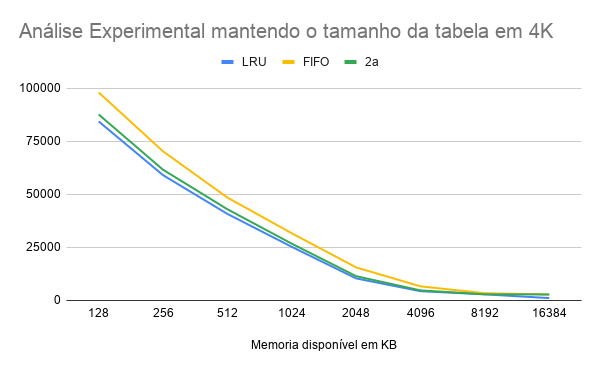
\includegraphics[scale=0.7]{Figuras/img2.png}
	\end{center}
	\caption{\label{fig:grafico2} }
\end{figure}

A análise visual, permite identificar uma aproximação de desempenho entre os métodos.
Porém é possível notar que \textit{FIFO} performou pior que os demais, uma vez que para
uma mesma quantidade de memória disponível e uma mesmo tamanho de página, esse método
possui um número maior de \textit{page faults}.
Porém, com o crescimento da quantidade de memória disponível, observou-se uma forte
aproximação do \textit{FIFO} com o método \textit{2A Chance} e há uma razão
por trás desse fato.
Ambos os algoritmos de reposição utilizam uma lista circular para apontar a próxima
pagina que será reposta no disco em caso de necessidade.
Entretanto, com diz o nome, \textit{2A Chance} aplica uma revalidação que dá a uma pagina
uma chance a mais de permanecer na lista.
Com uma memória disponível grande, a nova chance concedida às páginas não terá impacto
se comparado ao \textit{FIFO} tradicional.
Já o método \textit{LRU} possui um melhor desempenho que todos os algoritmos
independentemente do cenário, entretanto o à medida que a memória disponível cresce
o desempenho do \textit{LRU} também converge, juntamente com os outros dois métodos
de substituição de páginas.


\subsection{Variação do tamanho da página vs. Memória Constante}
Neste ultimo caso, apresentado na Figura \ref{fig:grafico3} mantivemos a quantidade
de memória constante em 512 Kilo Bytes e variamos o tamanho das páginas.
Assim como nos demais casos, das seções anteriores, os valore de \textit{page faults}
são referentes à media dentre os quatro arquivos de entrada fornecidos.
Comparando as Figura \ref{fig:grafico2} e \ref{fig:grafico3} o algoritmo
\textit{LRU} também possui
uma performance melhor do que os demais, sendo que \textit{2A Chance} tem 
comportamento semelhante, porém com um pequeno gap que a faz desse método menos
eficaz.


\begin{figure}[h]
	\begin{center}
		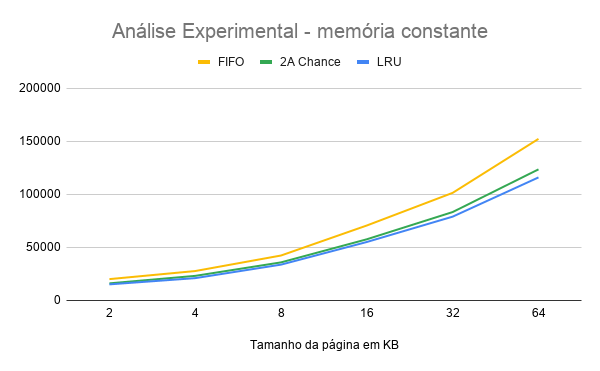
\includegraphics[scale=0.7]{Figuras/img3.png}
	\end{center}
	\caption{\label{fig:grafico3} }
\end{figure}

Na Figura \ref{fig:grafico3} também não incluímos o desempenho de \texttt{custom},
pois esse método se apresentou ineficaz e assim como na seção 4.1, a inclusão das
métricas desse gráfico atrapalharia a visualização das demais informações.
Outro fato que merece antenção é de que, em todos os gráficos observamos um aumento
na quantidade de \textit{page faults} à medida em que o tamanho da página aumenta.
Também há uma melhora de desempenho à medida em que a memória disponível aumenta.
O que demonstra uma dependência forte do desempenho dos algoritmos com o espaço
disponível.
Um possível algoritmo que conseguiria reduzir ou ter um impacto diferente destes
apresentados aqui, seria algum algoritmo preditivo, o qual alocaria as páginas
na memória baseado em fatores futuros, mas ainda assim haveria tal dependência.


% \section{Conclusão}
% \input{conclusion.tex}

% \begin{thebibliography}{9}

% \bibitem{cplusplus}
%     http://www.cplusplus.com 27 nov. 2019
    
% \bibitem{book:DFS}
%     Jon Kleinberg, Eva Tardos. 2006. \textit{Algorithm Design} (1st Edition, p 83). Pearson - Addison Wesley.
    
% \bibitem{book:BFS}
%     Jon Kleinberg, Eva Tardos. 2006. \textit{Algorithm Design} (1st Edition, p 79). Pearson - Addison Wesley.

% \bibitem{book:DAG}
%     Jon Kleinberg, Eva Tardos. 2006. \textit{Algorithm Design} (1st Edition, p 99 - 101). Pearson - Addison Wesley.
    
% \bibitem{cpp:vector}
%     http://www.cplusplus.com/reference/vector/vector 27 nov. 2019
    
% \bibitem{cpp:stack}
%     http://www.cplusplus.com/reference/stack/stack 27 nov. 2019
    
% \bibitem{cpp:iostream}
%     http://www.cplusplus.com/reference/iostream 27 nov. 2019
    
% \bibitem{cpp:chronos}
%     http://www.cplusplus.com/reference/chrono 27 nov. 2019
% \end{thebibliography}
\end{document}